%%%%%%%%%%%%%%%%%%%%%%%%%%%%%%%%%%%%%%%%%
% Beamer Presentation
% LaTeX Template
% Version 1.0 (10/11/12)
%
% This template has been downloaded from:
% http://www.LaTeXTemplates.com
%
% License:
% CC BY-NC-SA 3.0 (http://creativecommons.org/licenses/by-nc-sa/3.0/)
%
%%%%%%%%%%%%%%%%%%%%%%%%%%%%%%%%%%%%%%%%%

%----------------------------------------------------------------------------------------
%	PACKAGES AND THEMES
%----------------------------------------------------------------------------------------

\documentclass{beamer}

\mode<presentation> {

% The Beamer class comes with a number of default slide themes
% which change the colors and layouts of slides. Below this is a list
% of all the themes, uncomment each in turn to see what they look like.

%\usetheme{default}
%\usetheme{AnnArbor}
%\usetheme{Antibes}
%\usetheme{Bergen}
%\usetheme{Berkeley}
%\usetheme{Berlin}
%\usetheme{Boadilla}
%\usetheme{CambridgeUS}
%\usetheme{Copenhagen}
%\usetheme{Darmstadt}
%\usetheme{Dresden}
%\usetheme{Frankfurt}
%\usetheme{Goettingen}
%\usetheme{Hannover}
%\usetheme{Ilmenau}
%\usetheme{JuanLesPins}
%\usetheme{Luebeck}
\usetheme{Madrid}
%\usetheme{Malmoe}
%\usetheme{Marburg}
%\usetheme{Montpellier}
%\usetheme{PaloAlto}
%\usetheme{Pittsburgh}
%\usetheme{Rochester}
%\usetheme{Singapore}
%\usetheme{Szeged}
%\usetheme{Warsaw}

% As well as themes, the Beamer class has a number of color themes
% for any slide theme. Uncomment each of these in turn to see how it
% changes the colors of your current slide theme.

%\usecolortheme{albatross}
%\usecolortheme{beaver}
%\usecolortheme{beetle}
%\usecolortheme{crane}
%\usecolortheme{dolphin}
%\usecolortheme{dove}
%\usecolortheme{fly}
%\usecolortheme{lily}
%\usecolortheme{orchid}
%\usecolortheme{rose}
%\usecolortheme{seagull}
%\usecolortheme{seahorse}
%\usecolortheme{whale}
%\usecolortheme{wolverine}

%\setbeamertemplate{footline} % To remove the footer line in all slides uncomment this line
%\setbeamertemplate{footline}[page number] % To replace the footer line in all slides with a simple slide count uncomment this line

%\setbeamertemplate{navigation symbols}{} % To remove the navigation symbols from the bottom of all slides uncomment this line
}

\usepackage{graphicx} % Allows including images
\usepackage{booktabs} % Allows the use of \toprule, \midrule and \bottomrule in tables
\usepackage{amsmath}
\usepackage{verbatim}
\usepackage{tikz}
\usetikzlibrary{shapes.geometric, arrows}


%----------------------------------------------------------------------------------------
%	TITLE PAGE
%----------------------------------------------------------------------------------------

\title[Spectral learning with structure]{Spectral learning for structured partially observable environments} % The short title appears at the bottom of every slide, the full title is only on the title page

\author{Lucas Langer} % Your name
\institute[McGill University] % Your institution as it will appear on the bottom of every slide, may be shorthand to save space
{
%McGill University \\ % Your institution for the title page
Supervisors: Borja Balle, Doina Precup \\
\medskip
%\textit{lucas.langer@mail.mcgill.ca} % Your email address
}
\date{\today} % Date, can be changed to a custom date

\begin{document}


\begin{frame}
\titlepage % Print the title page as the first slide
\end{frame}

\begin{comment}
\begin{frame}
\frametitle{Overview} % Table of contents slide, comment this block out to remove it
\tableofcontents % Throughout your presentation, if you choose to use \section{} and \subsection{} commands, these will automatically be printed on this slide as an overview of your presentation
\end{frame}
\end{comment}


%----------------------------------------------------------------------------------------
%	PRESENTATION SLIDES
%----------------------------------------------------------------------------------------

%------------------------------------------------
\section{Predictive state representation (PSR)} % Sections can be created in order to organize your presentation into discrete blocks, all sections and subsections are automatically printed in the table of contents as an overview of the talk
%------------------------------------------------

%\subsection{Subsection Example} % A subsection can be created just before a set of slides with a common theme to further break down your presentation into chunks


%------------------------------------------------

\begin{frame}
\frametitle{Structured Partially Observable Environments}
\begin{columns}[c] % The "c" option specifies centered vertical alignment while the "t" option is used for top vertical alignment

\column{.45\textwidth} % Left column and width
\textbf{Structured Environments}
\begin{enumerate}
\item Goal: Predictions
\item Plan: Exploit structure
\item Example: Pacman

\end{enumerate}

\column{.5\textwidth} % Right column and width
\begin{figure}
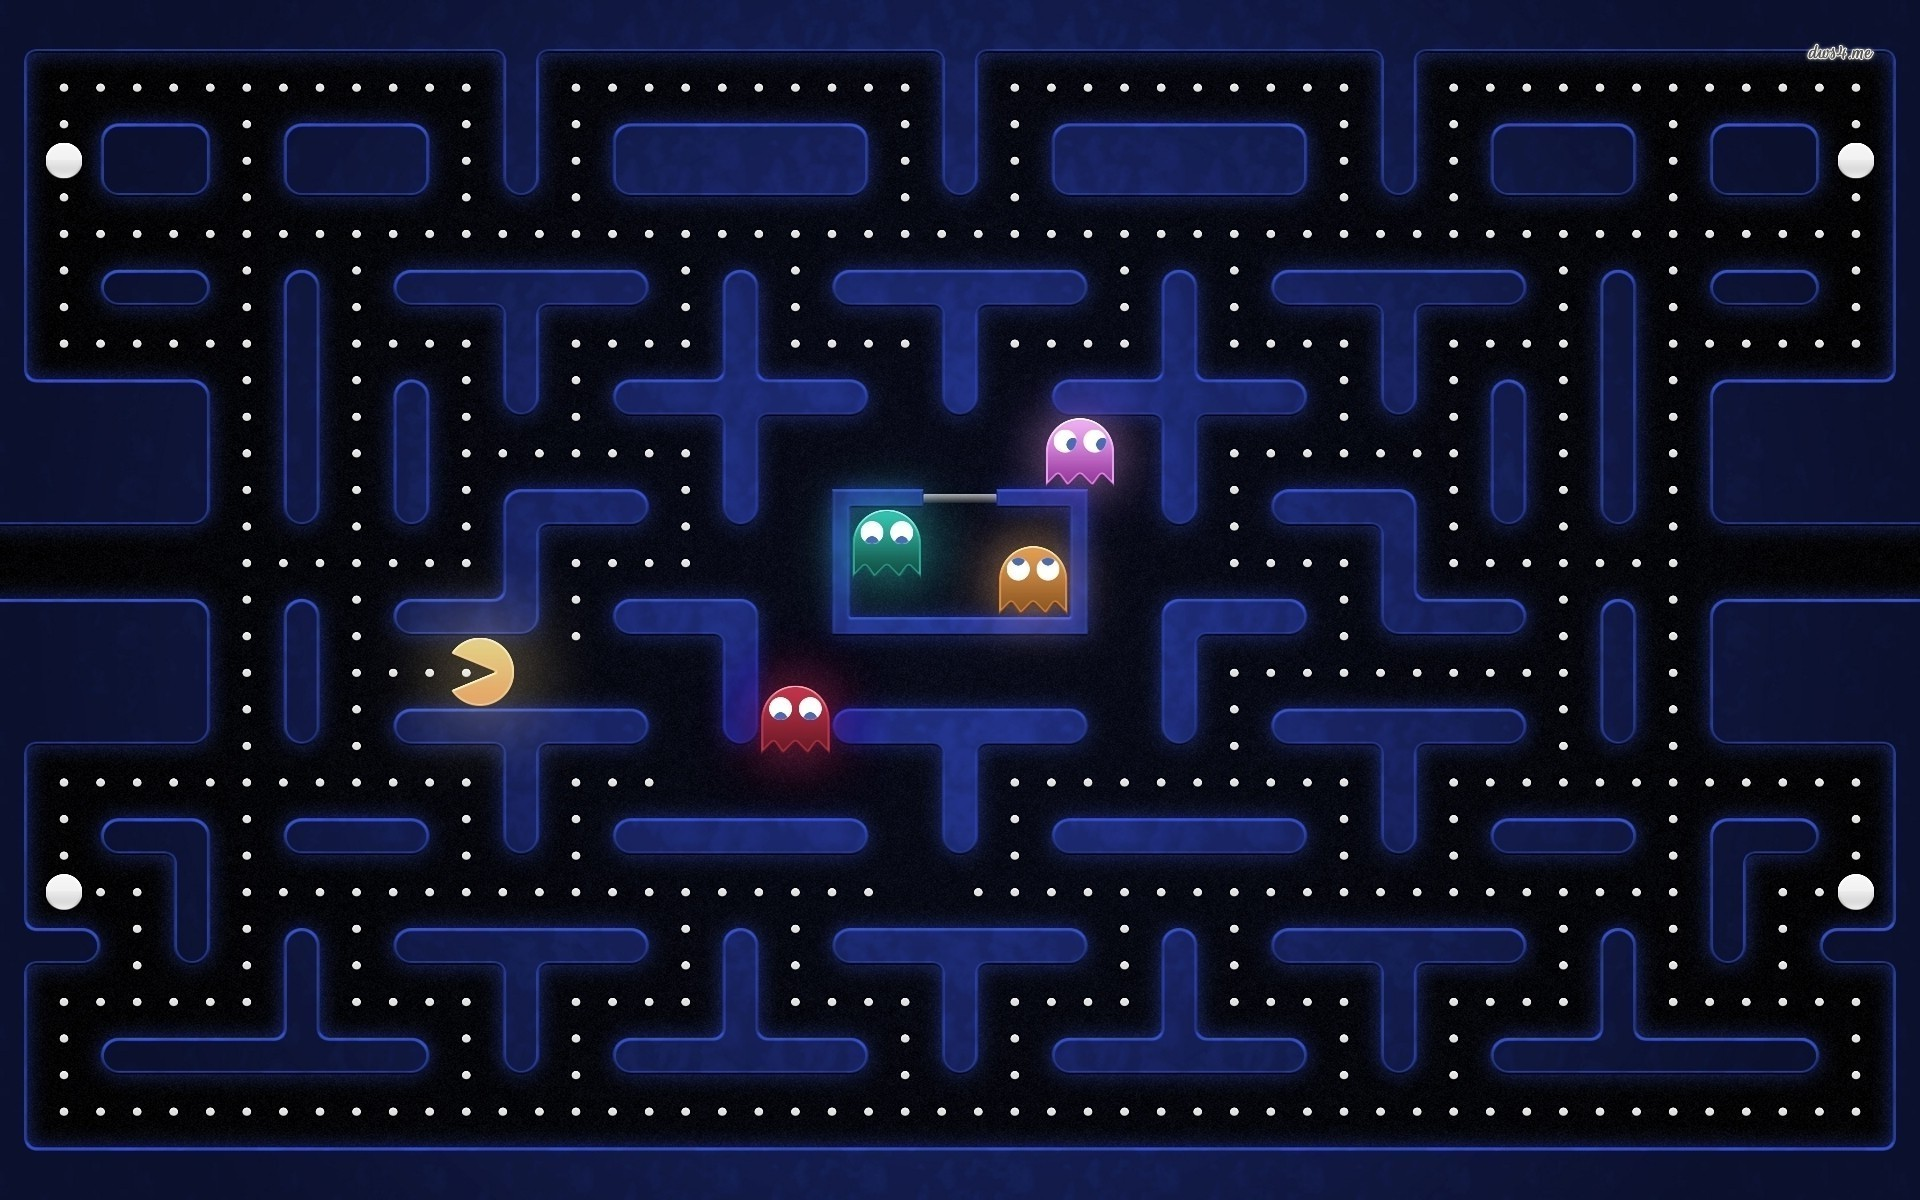
\includegraphics[width=1.0\linewidth]{lucasplots/pac-man.jpg}
\end{figure}

\end{columns}
\end{frame}

%------------------------------------------------

\begin{frame}
\frametitle{PSR: The Timing Case}

\begin{itemize}
\item Model environment with a Predictive state representation
\item For timing we have one observation symbol: {$\sigma$}
\item[] Notation: $\sigma$: one time unit, $\sigma^k$: k time units
\item[]
\item PSR defined by: $\langle \alpha_0, \{A_\sigma\},\alpha_\infty \rangle$
\item[] $\alpha_0$: Initial weighting on states $1xn$
\item[] $A_\sigma$: Transition matrix $nxn$
\item[] $\alpha_\infty$: Normalizer $nx1$
\item[]
\item PSRs compute probabilities of observations

\item[] $f(\sigma^k) = \alpha_0 \cdot A_\sigma^k \cdot \alpha_\infty$
 
\end{itemize}

\end{frame}

%------------------------------------------------

\begin{frame}
\frametitle{Spectral Learning of PSRs}

\begin{itemize}
\item[] Step 1: Represent data as a matrix
\item[] Step 2: Singular value decomposition
\item[] Step 3: Pick number of states for PSR
\item[] Step 4: Learn $\langle \alpha_0, \{A_\sigma\},\alpha_\infty \rangle$ with matrix computations
\end{itemize}

\end{frame}

\section{The Base System: extending PSRs}
%------------------------------------------------

\begin{frame}
\frametitle{The Base System}
\begin{itemize}

\item Idea: Add $\{A_{\sigma}, A_{\sigma^2}, A_{\sigma^4}, A_{\sigma^8}, ... A_{\sigma^N}\}$ as extra transition operators

\item Timing queries: $f(\sigma^{11}) = \alpha_0 \cdot A_{\sigma^8} \cdot A_{\sigma^2} \cdot A_{\sigma^1} \cdot \alpha_\infty$

\item Motivation: 
\item[] 1) Express transitions directly
\item[] 2) Faster queries
\end{itemize}
\end{frame}

%------------------------------------------------
\begin{comment}
\begin{frame}
\frametitle{The Base System Cont.}
\begin{itemize}

\item When taking a reduced model compounding errors are a threat

\item Analogy to rounding:  Round(51.63*34.12) v.s Round(51.63) * Round(34.12)

\item Let $\pi$: n states --> k states be the projection operator from a system with n states to the k-best states

\item
$f_Base(\sigma^128) = (\pi*\alpha_0)*(\pi*A_\sigma^128)*(\pi*\alpha_\infty)$

$f_Naive(x) = (\pi*\alpha_0)*(\pi*A_\sigma^128)*(\pi*\alpha_\infty)$ 

\end{itemize}

\end{frame}
\end{comment}

%------------------------------------------------


\section{Experimental results}
%------------------------------------------------

\begin{frame}
\frametitle{Timing with the Base}
Agent goes through loops until leaving through an exit state.  Loop lengths are 64 and 16 time units (not to scale).
\begin{figure}

\includegraphics[width=0.8\linewidth]{lucasplots/monImages/doubleLoopImage.png}
\end{figure}
\end{frame}

%------------------------------------------------
\begin{comment}


\begin{frame}
\frametitle{Varying amount of data}

\begin{itemize}
\item The \textbf{more data}, the \textbf{more effective} the Base System 
\item Left Figure: 10000 Trajectories
\item Right Figure: 250000 Trajectories

\end{itemize}


\begin{columns}[c]

\column{.5\textwidth} % Left column and width
\begin{figure}
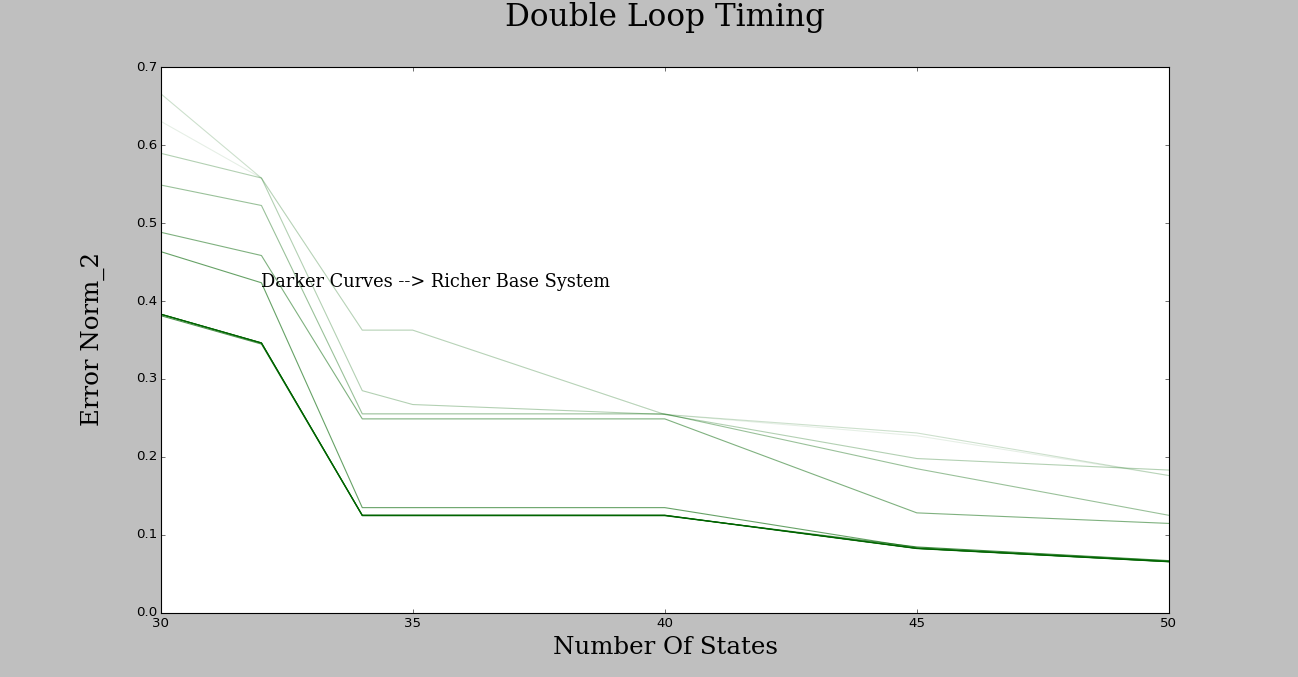
\includegraphics[width=1.0\linewidth]{lucasplots/monImages/DoubleLoopTiming0.png}
\end{figure}


\column{.5\textwidth} % Right column and width
\begin{figure}
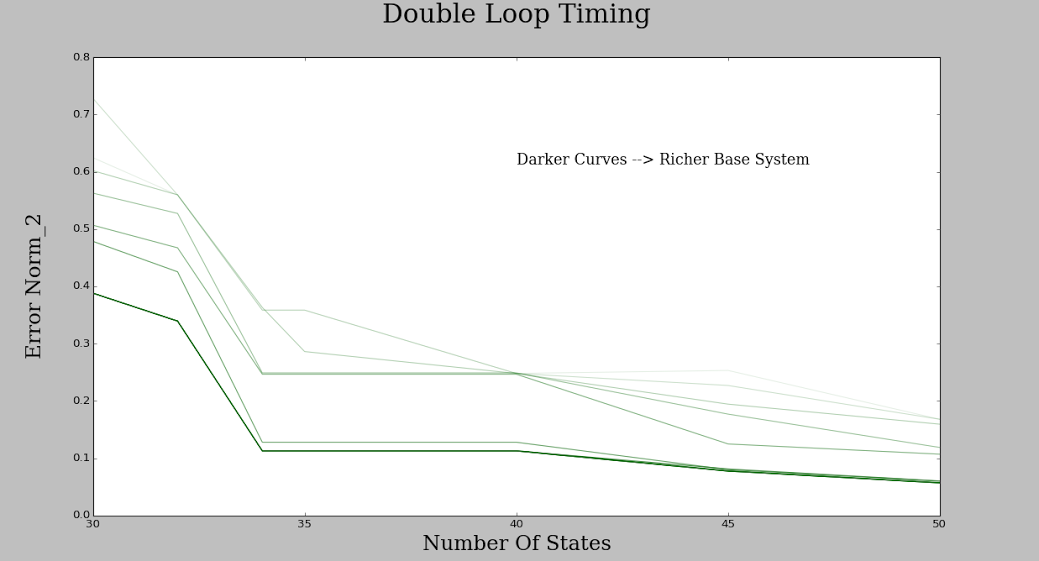
\includegraphics[width=1.0\linewidth]{lucasplots/monImages/highdata.png}
\end{figure}

\end{columns}

\begin{itemize}


\item[] $||f - \hat{f}|| = \sqrt{\sum\nolimits_{x \in observations}(f(x) - \hat{f(x)})^2}$ 
\end{itemize}


\end{frame}

\end{comment}
%------------------------------------------------


\begin{frame}
\frametitle{Base System Performance for Loops}


%\begin{itemize}
%\item Left Figure: No noise in durations
%\item Right Figure: Noise in loops

%\end{itemize}

\hspace{1cm} \textbf{No noise in durations}
\hspace{2.5cm} \textbf{Noise in durations}

\begin{columns}[c]

\column{.5\textwidth} % Left column and width
\begin{figure}

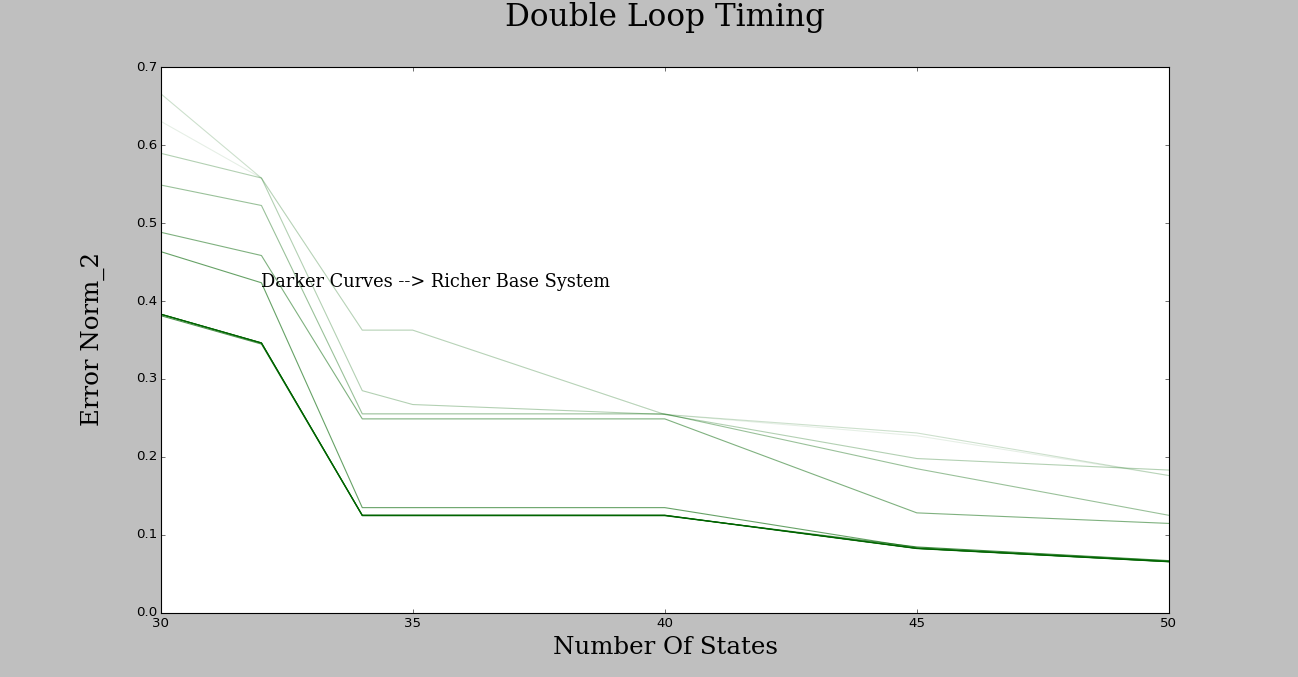
\includegraphics[width=1.0\linewidth]{lucasplots/monImages/DoubleLoopTiming0.png}
\end{figure}

\column{.5\textwidth} % Right column and width
\begin{figure}
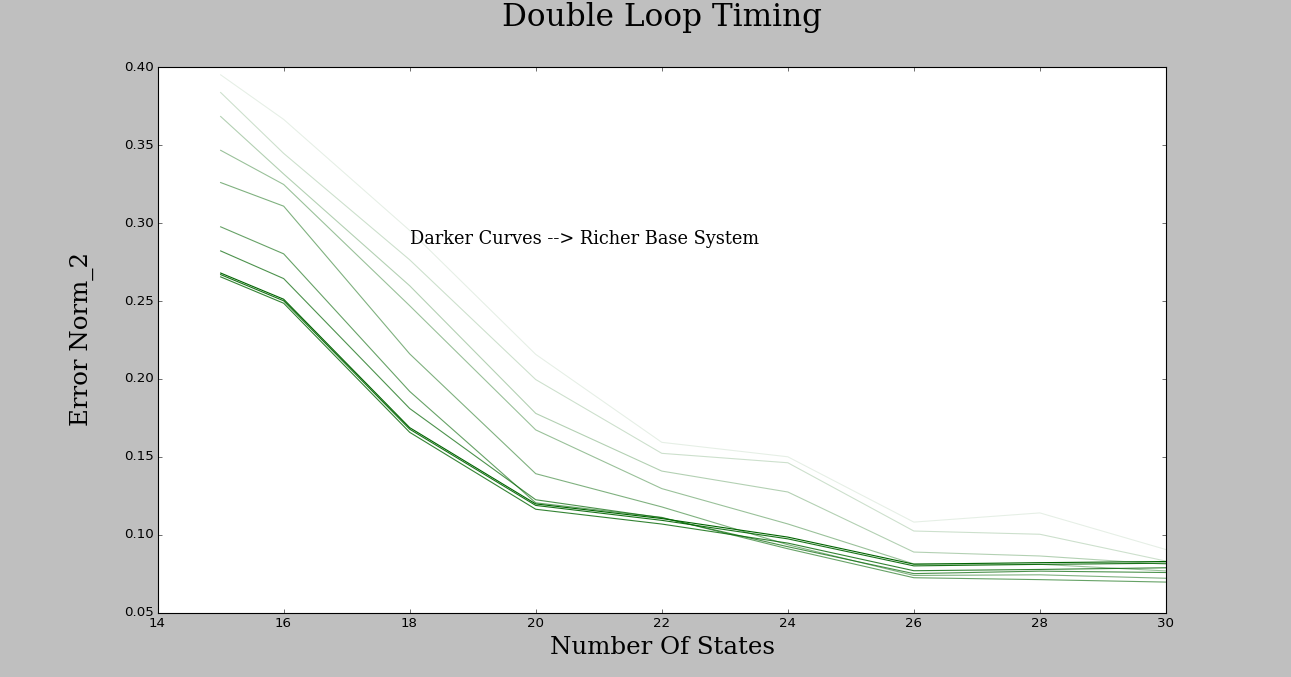
\includegraphics[width=1.0\linewidth]{lucasplots/monImages/DoubleLoopTiming0_1.png}
\end{figure}

\end{columns}

\begin{itemize}
\item Base System dominates for smaller models
\item Noise allows for smaller models

\item[] $||f - \hat{f}|| = \sqrt{\sum\nolimits_{x \in observations}(f(x) - \hat{f(x)})^2}$ 
\end{itemize}

\end{frame}

%------------------------------------------------


\begin{frame}
\frametitle{Pacman Labyrinth}

%\begin{itemize}
%\item Left figure: Timing predictions
%\item Right figure: Distance predictions
%\end{itemize}


\hspace{1cm} Timing Predictions
%\hspace{3cm} Distance Predictions

\begin{columns}[c]

\column{.55\textwidth} % Left column and width
\begin{figure}
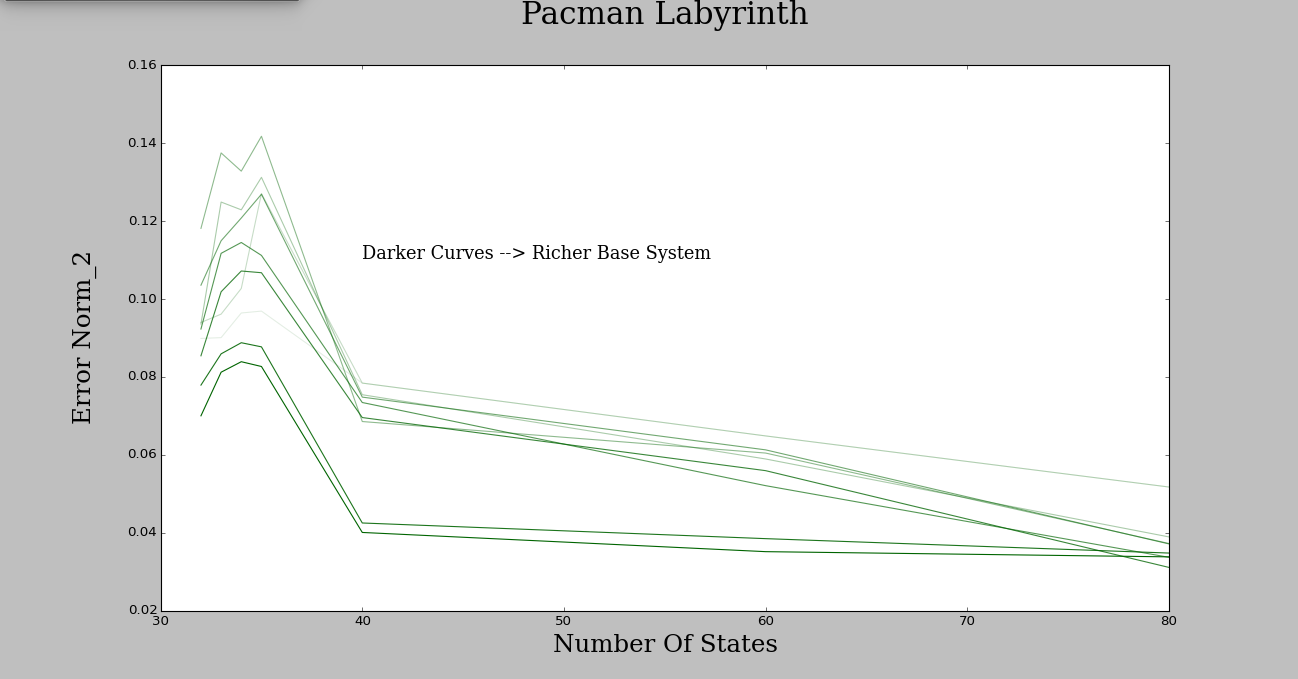
\includegraphics[width=1.0\linewidth]{lucasplots/monImages/PacmanLabyrinth.png}
\end{figure}


\column{.45\textwidth} % Right column and width
\begin{figure}
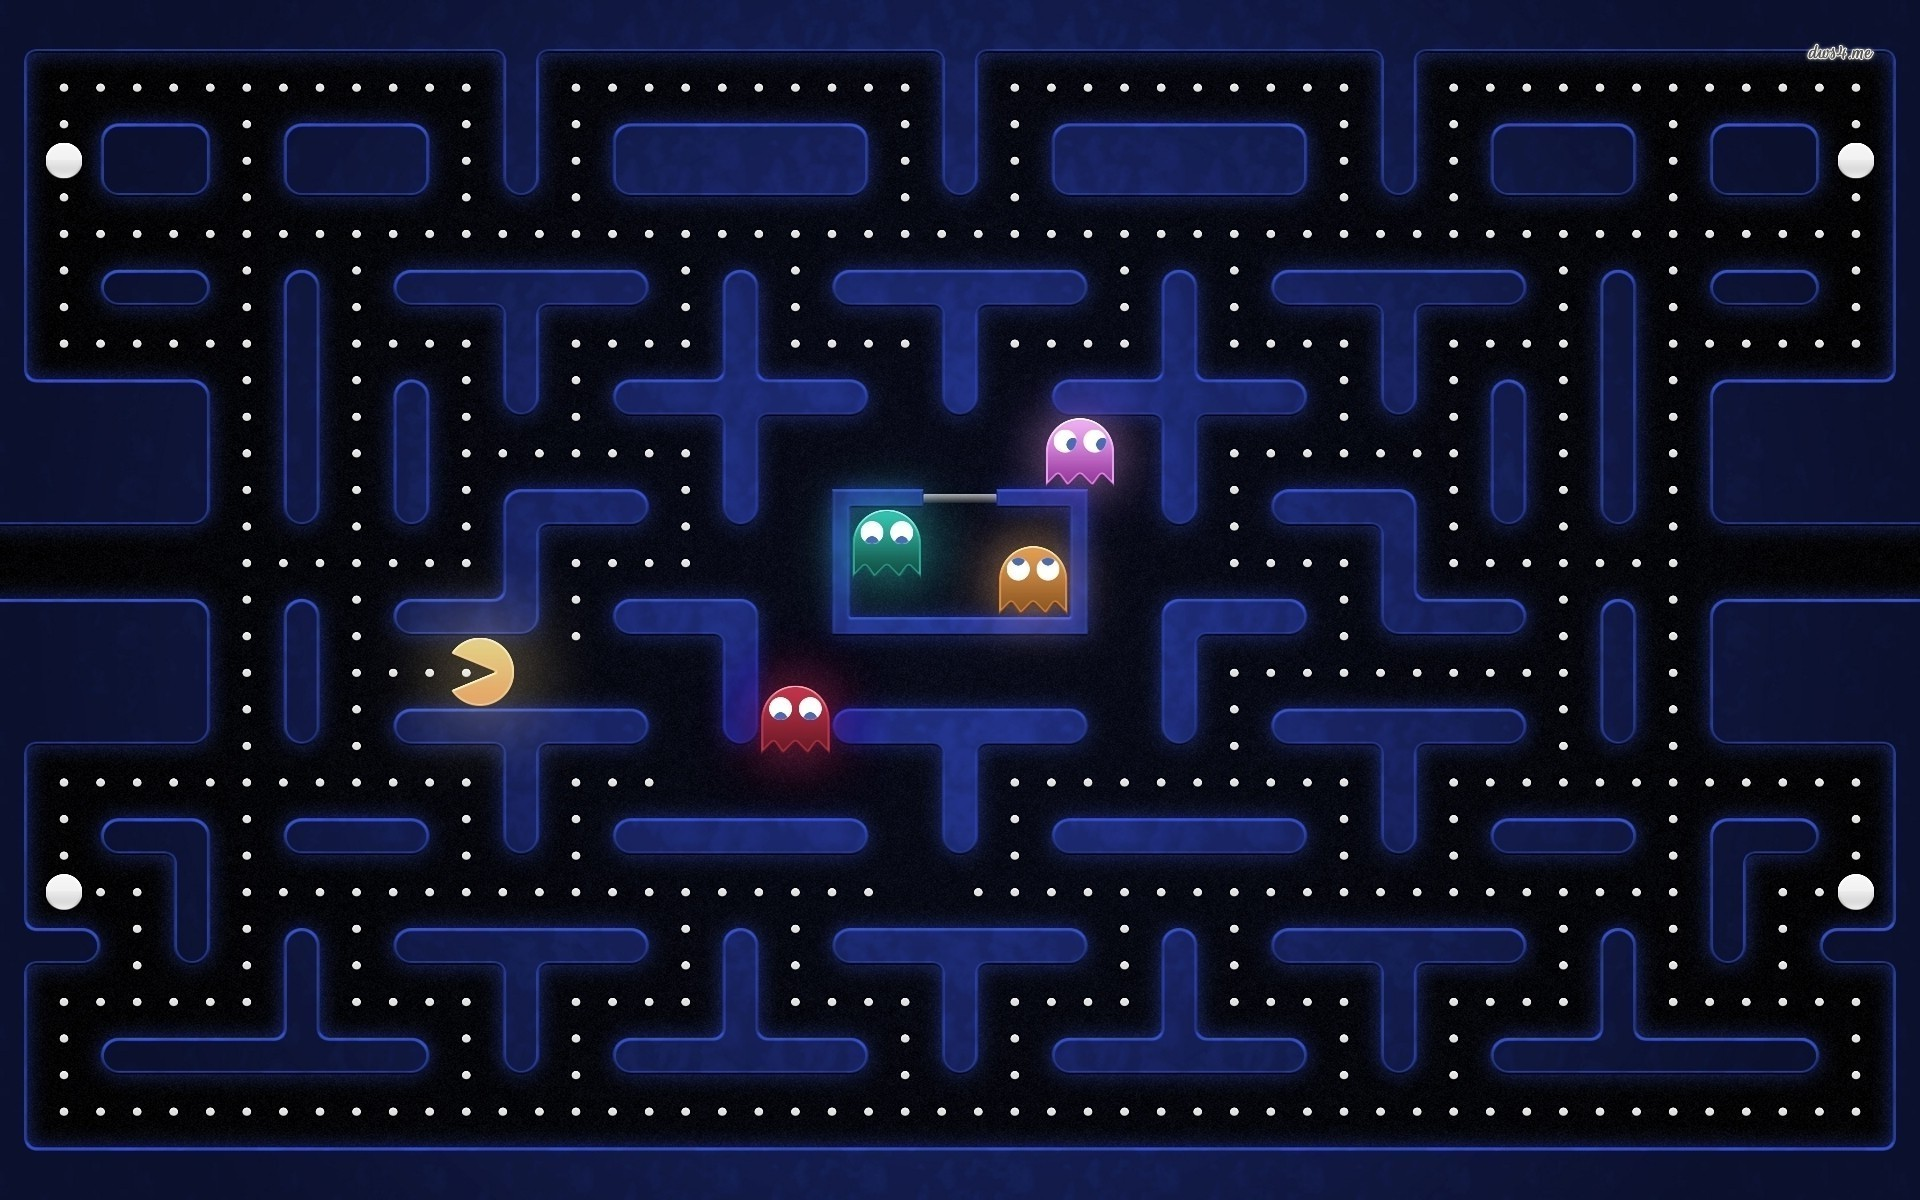
\includegraphics[width=1.0\linewidth]{lucasplots/pac-man.jpg}
\end{figure}

\end{columns}

\begin{itemize}

\item $||f - \hat{f}|| = \sqrt{\sum\nolimits_{x \in observations}(f(x) - \hat{f(x)})^2}$ 
\end{itemize}


\end{frame}

%------------------------------------------------

\begin{frame}
\frametitle{Wall Color Predictions}
We paint the first loop green and the second loop blue
\begin{figure}
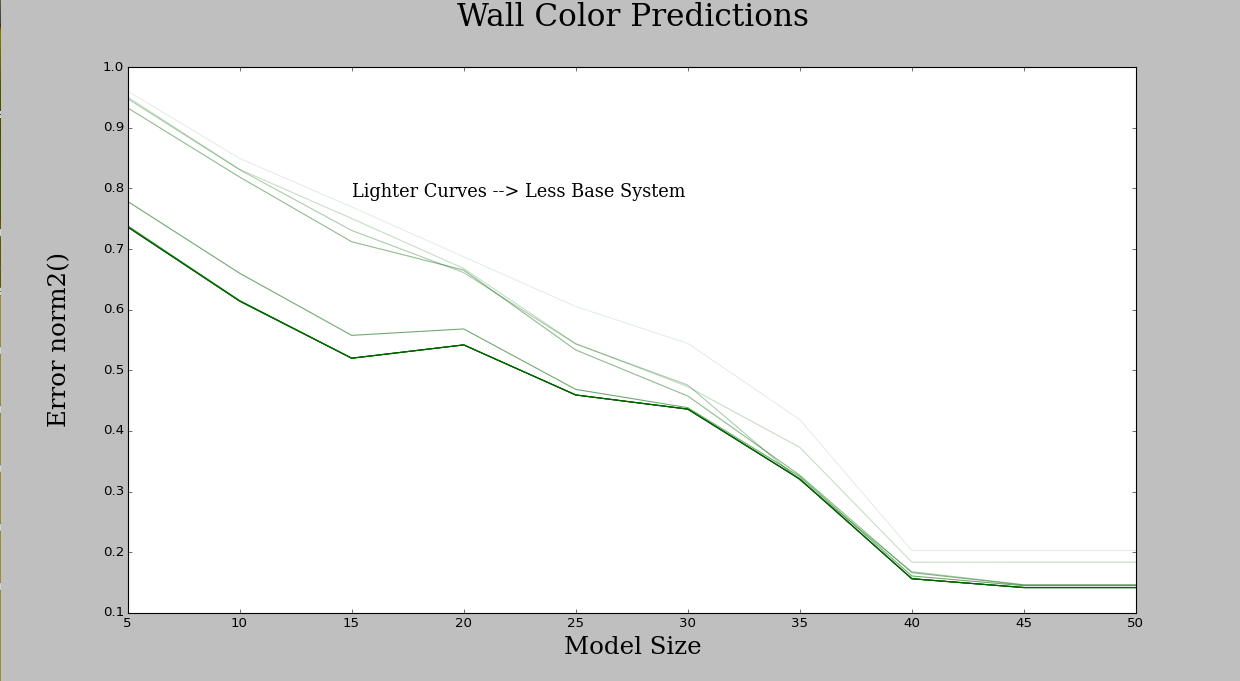
\includegraphics[width=0.6\linewidth]{lucasplots/monImages/WallColorPredictions.png}
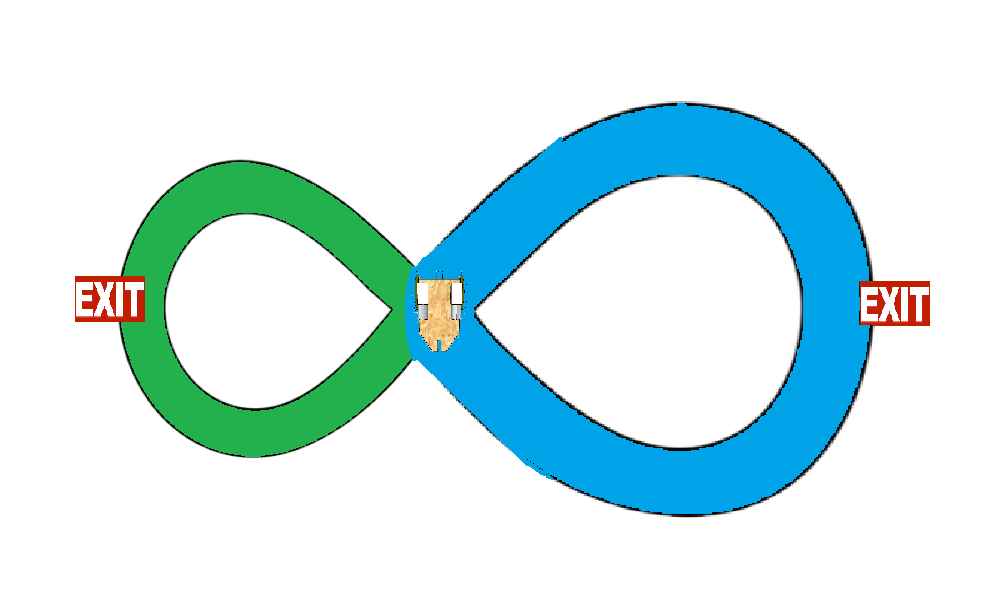
\includegraphics[width=0.4\linewidth]{lucasplots/monImages/doubleLoopImageMO.png}

\end{figure}

\begin{itemize}

\item[] $||f - \hat{f}|| = \sqrt{\sum\nolimits_{x \in observations}(f(x) - \hat{f(x)})^2}$ 
\end{itemize}

\end{frame}

%------------------------------------------------

%------------------------------------------------

\section{Learning the Base System}
%------------------------------------------------

\begin{frame}
\frametitle{Picking the Base System}
\begin{itemize}


\item Observations: \{"$a^{30}$":10, "$a^{60}$":5, "$b^{18}$":15\}

\item[] Desired Base System: $A_{a^{30}}$, $A_{b^{18}}$, $A_a$, $A_b$
\item[]

\item Solution: iterative greedy heuristic 
\item Substring properties: 
\textbf{long}, \textbf{frequent}, \textbf{diverse}
\item[]
\item Entropy view of structure


\end{itemize}
\end{frame}

%------------------------------------------------

\begin{frame}
\frametitle{Computing with the Base System}
\begin{itemize}


\item How should we execute queries?
\item[] Goal: \textbf{minimize number of matrices}
\item[]

\item[] Query string: "abcacb", Base System = $\{A_{ab}, A_{bca}, A_{cb}, A_a, A_b \}$ 


\item[] Desired partition: "a|bca|cb"
\item[] Computation: $f(abcacb)=\alpha_0 \cdot A_a \cdot A_{bca} \cdot A_{cb} \cdot \alpha_\infty$ 
\item[]

\item Solution: dynamic programming


\end{itemize}
\end{frame}

%------------------------------------------------

\begin{frame}
\frametitle{Conclusion and Future Work}
\begin{itemize}

\item What's left for the Base System?
\item[] 1) Theoretical analysis

\item[] 2) Test heuristics on labyrinths

\item[] 3) Further optimize heuristics


\end{itemize}
\end{frame}

%------------------------------------------------

\begin{frame}
\Huge{\centerline{Questions? Comments?}}
\end{frame}

\begin{frame}
\tikzstyle{startstop} = [rectangle, rounded corners, minimum width=3cm, minimum height=1cm,text centered, draw=black, fill=red!30]

\tikzstyle{io} = [trapezium, trapezium left angle=70, trapezium right angle=110, minimum width=3cm, minimum height=1cm, text centered, draw=black, fill=blue!30]

\tikzstyle{process} = [rectangle, minimum width=3cm, minimum height=1cm, text centered, draw=black, fill=orange!30]
\tikzstyle{decision} = [diamond, minimum width=3cm, minimum height=1cm, text centered, draw=black, fill=green!30]

\tikzstyle{arrow} = [thick,->,>=stealth]


\begin{tikzpicture}[node distance=2cm]

\node (start) [startstop] {Observation Data};

\node (in1) [io, below of=start] {Pick Operators};

\node (pro1) [process, below of=in1] {Learn Operators };
\node (dec1) [decision, below of=pro1] {PSR};

\node (pro2b) [process, right of=dec1, xshift=2cm] {Query String };
\node (out1) [io, right of=pro2b] {Optimal Partition};
\node (stop) [startstop, right of=out1] {Probability};

\draw [arrow] (start) -- (in1);
\draw [arrow] (in1) -- (pro1);
\draw [arrow] (pro1) -- (dec1);
\draw [arrow] (dec1) -- (pro2b);

\end{tikzpicture}
\end{frame}




%					DONE

%------------------------------------------------
%------------------------------------------------
%------------------------------------------------
%------------------------------------------------
%-----------------------------------------------
%------------------------------------------------
%------------------------------------------------

%					DONE


%----------------------------------------------------------------------------------------

\end{document} 